\documentclass{beamer}
\usetheme[titlepagelogo=crest,% Logo for the first page
						language=english
                        ]{TorinoTh}
                        
\usepackage[beamer,customcolors]{hf-tikz}
\hfsetfillcolor{alerted text.fg!10}
\hfsetbordercolor{alerted text.fg}

\author{James Friel}
\rel{Shay Cohen}
\title{Temporal Ordering of Historical
Events using Contextual Data}
\ateneo{Honours Project Presentation}
\date{\today}

\begin{document}
\titlepageframe

\begin{tframe}{Introduction}
  \begin{center}

    Is the use of contextual data useful to the temporal ordering of events?\vspace{1em}


    ``Alaska Becomes 49th US state''DD/MM/YYYY\vspace{1em}

    ``Manchester Shipping Canal Opens''DD/MM/YYYY\vspace{4em}
\end{center}
   Our dataset has 6224 of these.
\end{tframe}

\begin{tframe}{Related Work}
  Chambers \& Jurafsky (2009)-
  \begin{itemize}
    \item Unsupervised Learning of Event Relations
    \item Argument Representation
  \end{itemize}
  
  Abend et. al (2015) -
  \begin{itemize}
    \item Edge-factor models
    \item ILP \& Greedy Pathfinding
  \end{itemize}
  
  Mani et. al (2006) - 
  \begin{itemize}
    \item Hand Written \& Lexical Rules
    \item Ordering of Temporally Anchored Events
  \end{itemize}
  
\end{tframe}

\begin{tframe}{Information Extraction}
  Using OpenIE data extraction, extract subject, objects and relation
  \begin{center}
    \includegraphics[scale=0.3]{../openie-train.png}
  \end{center}
\end{tframe}
\begin{tframe}{Article Retrieval}
 Use Wikipedia API for article retrieval
\begin{minipage}{.5\textwidth}
\hspace{-1.25cm}
\centering
{\tiny
  \begin{enumerate}
  \item Extraction of only sentences that had a date within them
  \item Extraction of only sentences that had the other party in the relation within them
  \item Extraction of only sentences that had a date and the other party within them
  \item Extraction of paragraphs that referenced the other party
  \item Extraction of sentences that contained the object or the subject 
  \item Extraction of sentences that contained the object or the subject referenced the action between the two 
  \end{enumerate}
  }
\hspace{-1.25cm}
\end{minipage}%
\begin{minipage}{.5\textwidth}
\hspace{+0.25cm}
\centering
\begin{table}[H]
  \centering
  {\tiny
\begin{tabular}{|c|c|c|}
  \hline
Method & Average \# Sentences Retrieved & Relevancy \\
\hline
1      & 16                             &   -0.875  \\
2      & 2                              &   -1      \\
3      & 0.04                           &   0.5     \\
4      & 20                             &   -0.4    \\
5      & 27                             & -0.1\.{1}\\
6      & 32                             & 0.44\.{4}\\        
\hline
\end{tabular}
\caption{Retrieval Methods and their results}
\label{table:retrieval}
}
\end{table}
\end{minipage}
\end{tframe}

\begin{tframe}{Experiments}
  \begin{equation}
      \{(t_{i},s_{i},t_{j},s_{j},b_{ij})\} \hspace{0.5em} \text{for} \hspace{0.5em} i,j \hspace{0.2em}\in \hspace{0.2em}[M]\nonumber
    \end{equation}
  where $b_{ij} = [y_{i} > y_{j}]$ indicates which event came first.
  $T_*$ is a title.
  $S_*$ is the retrieved sentences.\vspace{1em}
  
  From this we train various different classifiers:
  \begin{itemize}
  \item Decision Tree
  \item SVM
  \item Logistic Regression
  \item Perceptron
  \item Multilayer Perceptron
    \end{itemize}
\end{tframe}


\begin{tframe}{Results - Classifiers}
\begin{table}[H]
\centering
\begin{tabular}{|c|c|c|c|c|c|c|c|}
  \hline
  Accuracy  & DT  & SVM & LR & Perceptron & MLP & Baseline\\
  \hline
  With Articles    & 53\%   & 66\% &  76\% & 66\% & 83\% & $\frac{1}{2^{622}}$\%\\
\hline
With Titles & 43\%  & 51\%    & 52\% & 46\% & 54\% & $\frac{1}{2^{622}}$\%\\
\hline
\end{tabular}
\caption{Classification Results for Tuples}
\label{table:classification-results}
\end{table}

\begin{table}[H]
\centering
\begin{tabular}{|c|c|c|c|c|c|c|}
  \hline
  Accuracy  & DT & SVM & LR & Perceptron & MLP & Baseline\\
  \hline
  With Articles & 13\%    & 13\% &  23\% & 27\% & 21\% &  $\frac{1}{4^{622}}$\%\\
\hline
With Titles & 21\% & 13\%    & 24\% & 33\% & 14\% &  $\frac{1}{4^{622}}$\%\\
\hline
\end{tabular}
\caption{Classification Results for Triples}
\label{table:triple-classification-results}
\end{table}
\end{tframe}

\begin{tframe}{Results - Tuples}
\begin{table}[H]
\centering
\begin{tabular}{|c|c|c|c|c|c|c|c|}
  \hline
  A$*$ Search & DT & SVM &LR & Perceptron & MLP & Baseline\\
  \hline
With Articles & 0.695 & 0.419 & 0.3 & 0.376   & 0.7333  & 0\\
\hline
With Titles &0.06  & -0.09 & 0.048 & -0.52  & -0.28 & 0\\
\hline
\end{tabular}
\caption{ILP Pathing Results for Tuples}
\label{table:ILP-results}
\end{table}

\begin{table}[H]
\centering
\begin{tabular}{|c|c|c|c|c|c|c|c|}
  \hline
  Beam Search & DT & SVM &LR & Perceptron & MLP & Baseline\\
  \hline
With Articles & 0.42 & 0.5151 & 0.3 &  0.44  & 0.5454  & 0\\
\hline
With Titles & 0.214 & -0.62 & 0.17 & 0.09  & 0.32 & 0\\
\hline
\end{tabular}
\caption{Greedy Pathing Results for Tuples}
\label{table:greedy-results}
\end{table}

\end{tframe}
\begin{tframe}{Results - Triples}

\begin{table}[H]
\centering
\begin{tabular}{|c|c|c|c|c|c|c|c|}
  \hline
  A$*$ Search & DT & SVM &LR & Perceptron & MLP & Baseline\\
  \hline
With Articles & -0.64 & -0.54 & -0.92 & -0.53   & -0.58  & 0\\
\hline
With Titles & -0.62  & -0.68 & -0.87 & -0.61  & -0.59 & 0\\
\hline
\end{tabular}
\caption{ILP Pathing Results for Triples}
\label{table:ILP-results-triple}
\end{table}

\begin{table}[H]
\centering
\begin{tabular}{|c|c|c|c|c|c|c|c|}
  \hline
  A$*$ Search & DT & SVM &LR & Perceptron & MLP & Baseline\\
  \hline
With Articles & -0.64 & -0.54 & -0.92 & -0.53   & -0.58  & 0\\
\hline
With Titles & -0.62  & -0.68 & -0.87 & -0.61  & -0.59 & 0\\
\hline
\end{tabular}
\caption{ILP Pathing Results for Triples}
\label{table:ILP-results-triple}
\end{table}

\end{tframe}

\begin{tframe}{Graphs}
  \begin{center}
    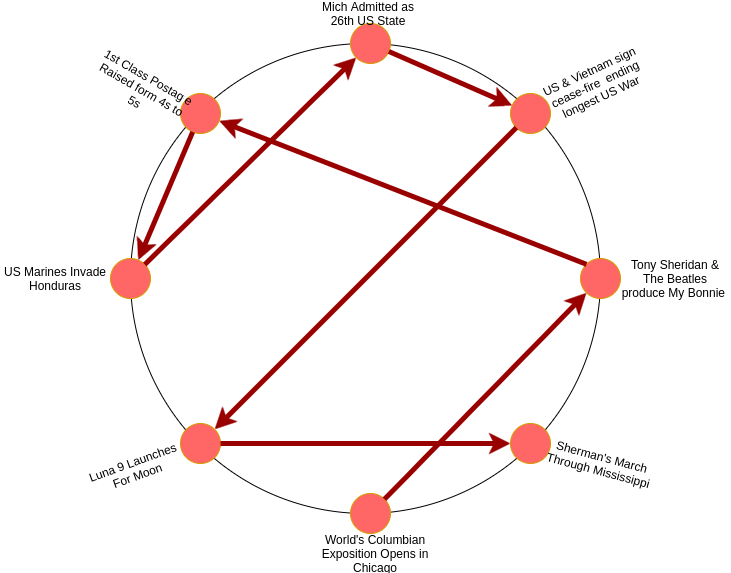
\includegraphics[scale=0.3]{../node-graph.png}
  \end{center}
 \end{tframe}

\begin{tframe}{Conclusion}
  \begin{center}
    \begin{itemize}
    \item Use of external data source provide up to 30\% better accuracy
    \item Multiplayer Perceptron with ILP proved best - 83\% Accuracy
    \item Further improvments can build upon this work  
    \end{itemize}
  \end{center}
\end{tframe}
\end{document}
